\section{Analysis Techniques}
\label{sec:Analysis}

\subsection{Handling Time}
\label{handling_time}

The CPN-based analysis consists of executing a simulation of the model and constructing a state space data structure for the system (for a finite horizon), and then performing queries on this data structure. This is automated by CPN Tools. The first improvement over the basic CPN approach is in how we handle time. Although it is true that CPN and similar extensions to Petri Nets such as Timed Petri Nets inherently have modeling concepts for simulation time, we explicitly model time as an integer-valued \emph{clock} color token in CPN. There are several reasons for this choice. 

Firstly, this is an extension to our previous arguments about choosing Colored Petri Nets. Modeling the OS scheduler clock as a colored token allows for extensions to its data structure such as (1) intermediate time stamps and internal state variables, and (2) adding temporal partitioning schemes like the (time-partitioned) ARINC-653 \cite{ARINC-653} scheduling model (Figure \ref{fig:clock}). These extended data structure fields can be more easily manipulated and used by the model transitions during state changes, allowing for richer modeling concepts that would not be easily attainable using token representations provided by Timed Petri Nets. The ability to pack colored tokens with rich data structures also reduces the total number of colors required by the complete model. This quantitative measure directly influences the reduced size of the resultant state space. The downside of this approach to modeling is that we have to choose a time quantum. But in practical systems this is usually not a problem, as the low-level scheduling decisions are taken by an OS scheduler based on a time scale with a finite resolution. We have chosen 1 msec as the quantum (corresponding to the typical 1KHz scheduler in Linux), but it can be easily changed. 

\vspace{-0.1in}
\begin{figure}[h]
	\centering
	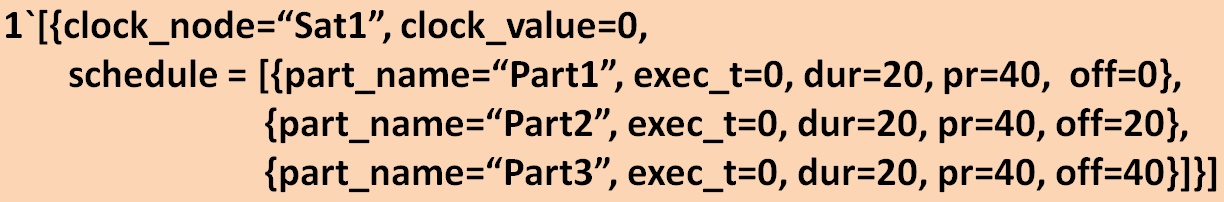
\includegraphics[width=0.5\textwidth]{./figs/clock}
	\caption{A Clock Token with Temporal Partitioning}
	\label{fig:clock}
\end{figure}

Secondly, modeling time as a token allows for smarter time progression schemes that can be applied to control the pace of simulation. If we did not have such control over time, the number of states recorded for this color token would eventually explode and itself contribute to a large state space. In order to manage this complexity, we have devised some appropriate \emph{time jumps} in specific simulation scenarios. 

If the rate at which time progresses does not change, then for a 1 msec time resolution, \emph{S} seconds of activity will generate a state space of size: $SS_{size} = \sum\limits_{i=1}^{S*1000} TF_{t_i}$ where $TF_{t_i}$ is the number of state-changing CPN transition firings between $t_i$ and $t_{i+1}$. This large state space includes intervals of time where there is no thread activity to analyze either due to lack of operation requests, lack of ready threads for scheduling, or due to temporal partitioning. During such idle periods, it is prudent to allow the analysis engine to \emph{fast-forward} time either to (1) the next node-specific clock tick, (2) the next global timer expiry event, or (3) the next activation of the node-specific temporal partition (whichever is earliest and most relevant). This ensures that the generated state space tree is devoid of nodes where there is no thread activity.

\begin{figure}[h]
	\centering
	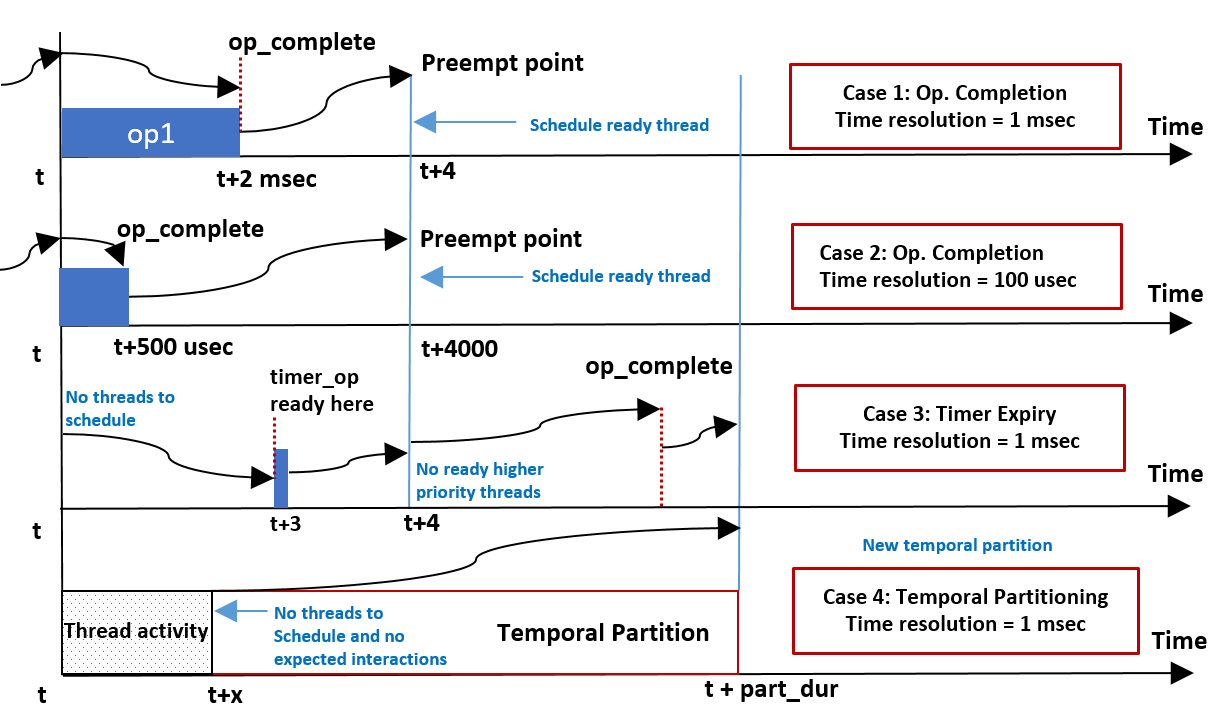
\includegraphics[width=0.5\textwidth]{./figs/time}
	\caption{Dynamic Time Progression}
	\label{fig:time}
\end{figure}

Figure \ref{fig:time} illustrates these time jumps using 4 scenarios. Assuming the scheduler clock ticks every 4 msec, Case 1 shows how time progression is handled when an operation completes 2 msec into its thread execution. At time t, the model identifies the duration of time left for an operation to complete. If this duration is earlier than the next preempt point, then there is no need to progress time in 1 msec increments as no thread can preempt this currently running thread till time t + 4 msec. Therefore, the \emph{clock\_value} in Figure \ref{fig:clock} progresses to time t + 2 msec, where the model handles the implications of the completed operation. This includes possibly new interactions and operation requests triggered in other components. Then, time is forced to progress to the next preempt point where a new candidate thread is scheduled. This same scenario is illustrated in Case 2 when the time resolution is increased to 100 usec instead of 1 msec. Notice that the number of steps taken to reach the preempt point are the same, showing how the state space doesn't have to explode simply because the time resolution is increased. Case 3 illustrates the scenario where at time t, the scheduler has no ready threads to schedule since there are no pending operation requests but at time t + 3 msec, a component timer expires, triggering an operation into execution. Since timers are maintained in a global list, each time the \emph{Progress\_Time} transition checks its firing conditions, it checks all possible timers that can expiry before the next preempt point. So, at time t when no threads are scheduled, the model immediately jumps to time t + 3. This scenario also shows that if the triggered operation does not complete before the preempt point \emph{and} there are no other ready threads or timer expiries that can be scheduled, the clock value jumps to the operation completion. It must be noted here that this case is valid only because the DREMS architecture we have considered uses a non-preemptive operation scheduling scheme. Lastly, Case 4 shows time jumps working with temporal partitioning. At some time t + x, the model realizes the absence of ready threads and does not foresee any interaction requests from other components, then it safely jumps to the end of the partition without stepping forward in 1 msec increments. This time progression directly shows how the state space of the system execution reduces while still preserving the expected execution order, justifying our choice of modeling time as a colored token using CPN. 

\subsection{Distributed Deployment} 
\label{distributed_deployment}

The second structural change to the analysis model is in how distributed deployments are modeled and simulated. Early designs on modeling and analysis of distributed application deployments \cite{MoDeVVa} included a unique token per CPN place for each hardware node in the scenario. Since the individual \emph{node} tokens are independent and unordered, there is nondeterminism in the transition bindings when choosing a hardware node to schedule threads in. For instance, if there are 2 hardware nodes in the deployment with ready threads on both nodes, then either node can be chosen first for scheduling threads leading to two possible variations of the model execution trace. Therefore the generated state space would exponentially grow for each new hardware node. In order to reduce this state space and improve the search efficiency, we have merged hardware node tokens into a single \emph{list} of tokens instead of a unassociated grouping of individual node tokens. This approach is inspired by the symmetry method for state space reduction \cite{Kristensen2000}.

\begin{figure}[h]
	\centering
	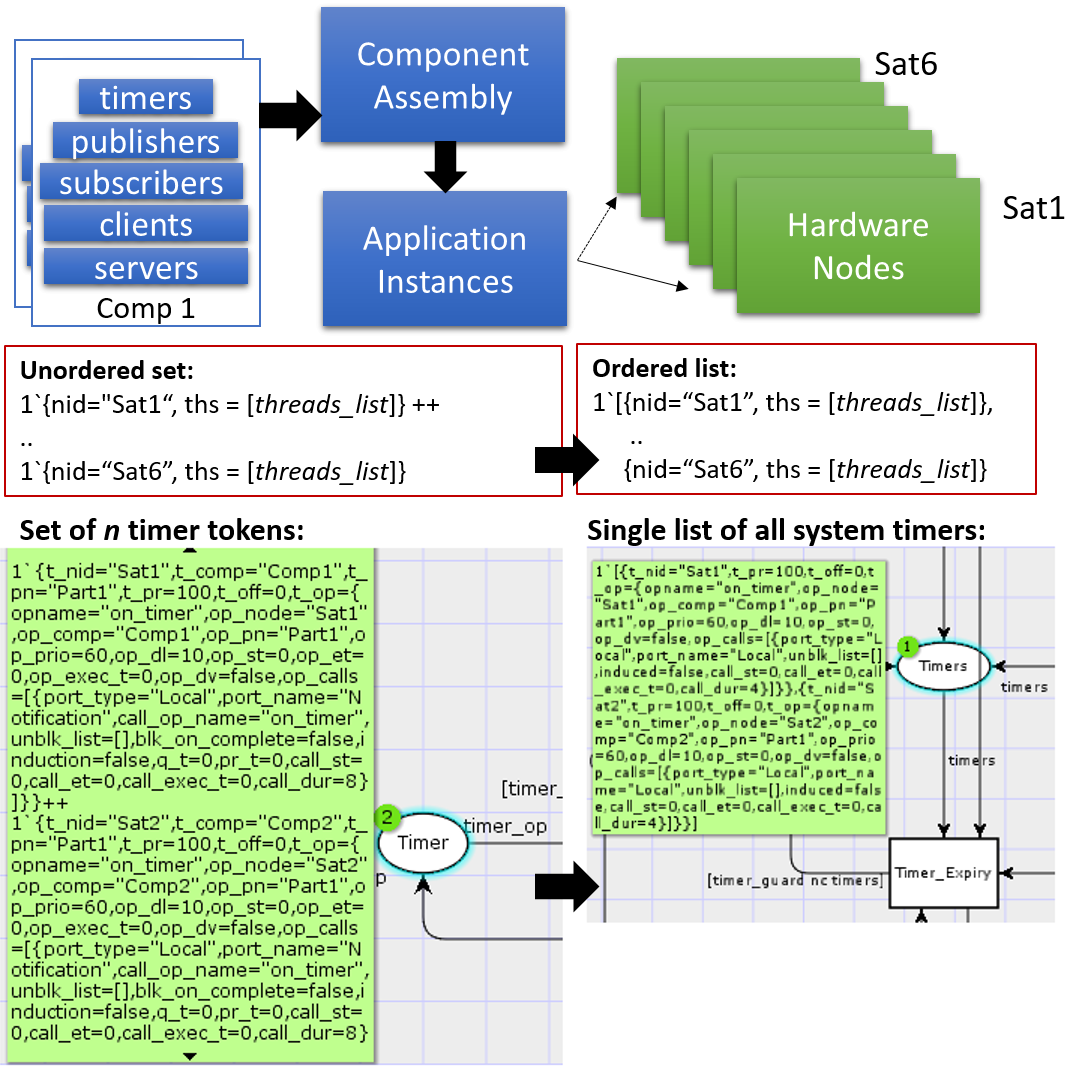
\includegraphics[width=0.5\textwidth]{./figs/dd}
	\caption{Structural Reductions in CPN}
	\label{fig:dd}
\end{figure}

Figure \ref{fig:dd} illustrates this structural reduction. Consider a distributed deployment scenario with an instance of a DREMS application deployed on each hardware node, Sat1 through Sat6. Components \emph{Comp1} and \emph{Comp2} are triggered by timers, eventually leading to the execution of component operations (modeled as shown in Figure \ref{fig:ebnf}). If all the timer tokens in the system were modeled individually, the transition \emph{Timer\_Expiry} would non-deterministically choose one of the two timer tokens that are ready to expire at \emph{t=0}. However, if the timers are maintained as a single list, then this transition (1) consumes the entire list, (2) identifies all timers that are ready to expire, (3) evaluates the timer expiration function on all ready timers, (4) propagates the output \emph{operation} tokens to the relevant component message queues in a single firing. This greatly reduces the tree of possible transition firings and therefore the resultant state space. Also, if there is no non-determinism in the entire system, i.e., there is a distinct ordering of thread execution, then this model can be scaled up with instantiating the application on new hardware nodes with no increase in state space size. This is because all of the relevant tokens on all nodes are maintained as a single list that is completely handled by a single transition firing. 

An important implication of the above structural reduction is that the simulation of the entire system now progresses in synchronous steps. This means that at time 0, all the timers in all hardware nodes that are ready to expire will expire in a single step. Following this, all operations in all component message queues of all these nodes are evaluated together and appropriate component executor threads are scheduled together. When these threads execute, time progresses as described in Section \ref{handling_time}, moving forward by the minimum amount of time that can be fast-forwarded.

\subsection{Advanced State Space Analysis Methods}

State space analysis techniques have been successfully applied with Colored Petri Nets in a variety of practical scenarios and industrial use cases \cite{CPN_0}, \cite{CPN_1}. The basic idea here is to compute all reachable states of the modeled concurrent system and derive a directed graph called the \emph{state space}. The graph represents the tree of possible executions that the system can take from an initial state. It is possible from this directed graph to verify behavioral properties such as queue overflows, deadline violations, system-wide deadlocks and even derive counterexamples when arriving at undesired states. 

The variety of CPN-specific state space reduction techniques \cite{CPN_Sweepline}, \cite{CPN_Symmetry} developed in recent times has significantly broadened the class of systems that can be verified. In order to easily apply such techniques to our analysis model, we use the ASAP \cite{ASAP} analysis tool. The tool provides for several search algorithms and state space reduction techniques such as the \emph{sweep-line method} \cite{Christensen2001} which deletes already visited state space nodes from memory, forcing on-the-fly verification of temporal properties. The main advantage of such a technique is the amount of memory required by the analysis to verify useful properties for large models. 

\begin{figure*}[ht]
	\centering
	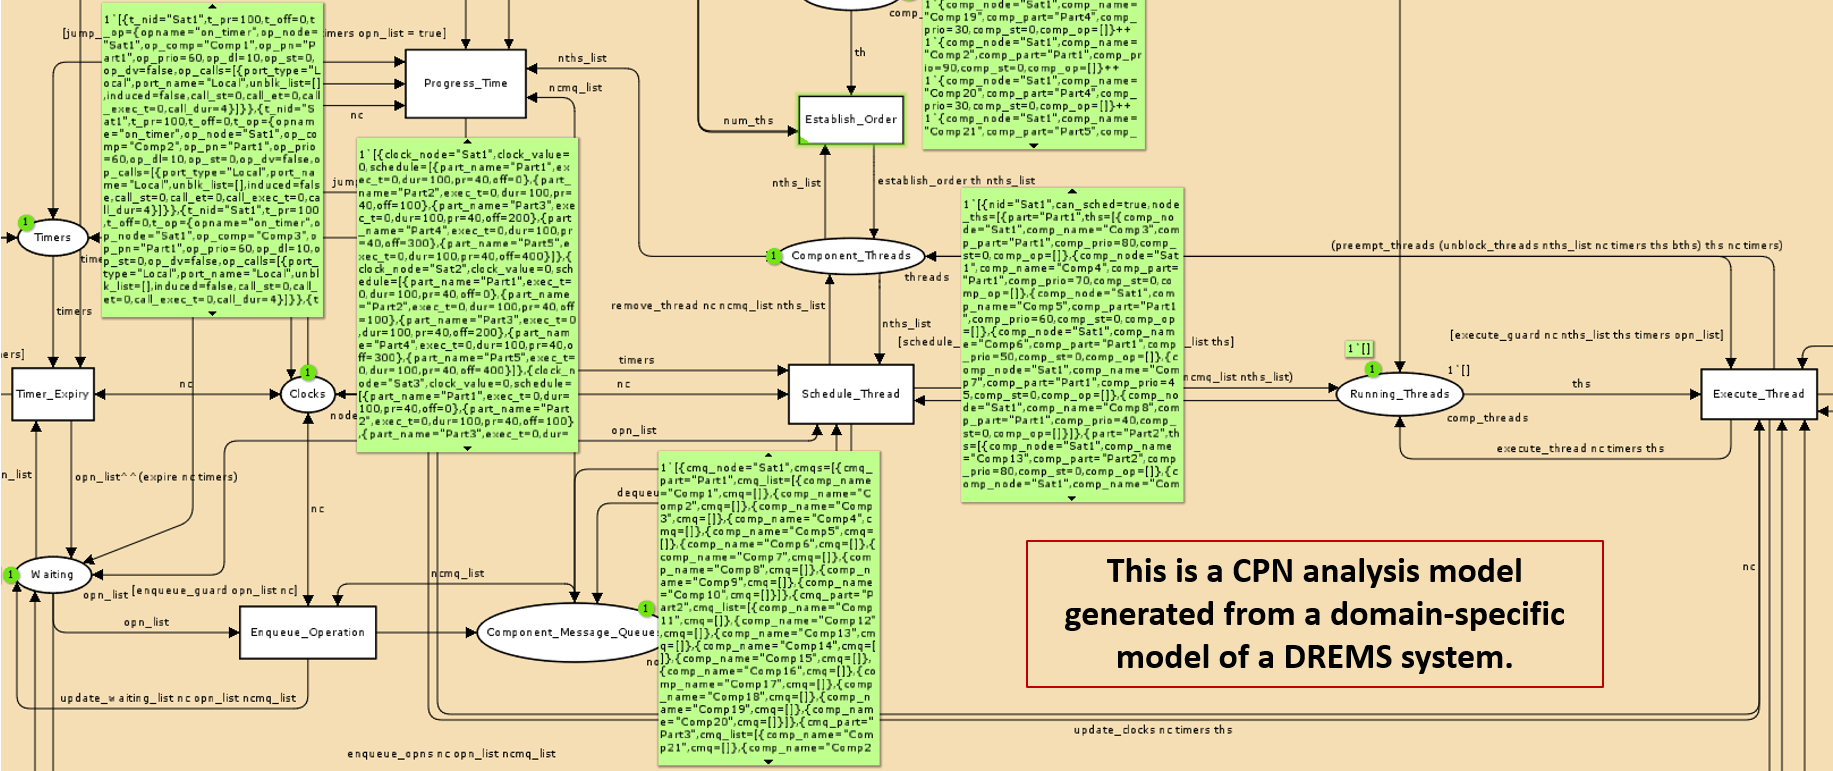
\includegraphics[width=\textwidth]{./figs/Generated_Model}
	\caption{Generated CPN model for a Distributed Application Deployment}
	\label{fig:gm}
\end{figure*}

The sweep line method for state space reduction is used to check for important safety properties such as lack of deadlocks, timing violations etc. using user-defined model-specific queries. Practical results enumerated in \cite{Christensen2001} show improvements in time and memory requirements for generating and verifying bounded state spaces. The method relies of discarding generated states on-the-fly by performing verification checks during state space generation time. Any state that does not violate system properties can be safely deleted. Another advantage of this method of similar reduction methods such as bit-state hashing \cite{CPN_Bitstate_Hashing} is that a complete state space search is guaranteed. 

In order to illustrate the utility of such state space reduction techniques, we consider a large-scale deployment. Figure \ref{fig:gm} shows the generated CPN model for a domain-specific DREMS application. This is a scaled-up variant of several satellite cluster examples we have used in previous publications \cite{DREMS13Software}, \cite{MoDeVVa}. The example consists of a group of communicating satellites hosting DREMS applications. The component assembly for this application consists of 100 interacting components distributed across 10 computing nodes, many of which are triggered by infrastructural timers. Notice in Figure \ref{fig:gm} how there is only one token in each of the main CPN places, as described in Section \ref{distributed_deployment}. All of the component timers are appended to the list maintained in \emph{Timers} place. Similarly, all node-specific clock tokens are maintained in place \emph{Clocks}.  

At time \emph{t=0}, before the simulation is kicked off, the transition \emph{Establish\_Order} generates the powerset of thread execution orders that are possible given the configuration of the clock token. This may be a potentially large set depending on the number of threads of equal priority in each partition. Once this tree of possible orders is established, the complete set of timers that are ready to expire are evaluated. Each timer expiry manifests as an operation request and each callback operation modeled using the grammar shown in Figure \ref{fig:ebnf}. Once the operations are ready to execute, the highest priority component thread with a pending operation request is chosen for execution. This thread scheduling happens on all hardware nodes. When each thread executes, new interactions may occur as a consequence of the execution. For instance, if a component thread executes a timer operation in which the component publishes on a global topic, the consequence of this action would include a set of callback operation requests on all components that contain subscribers to that global topic. Lastly, all running threads are evaluated to identify the minimum amount of time that can be safely fast-forwarded in each node. If the running component threads are independent or symmetrical, then the maximum possible time progression is up to the end of the temporal partition. Note here that temporal partition in the deployment can be set to an empty list which simply removes the  partitioning constraint and treats all component threads on a node as candidate threads for execution. The above sequence of transitions repeat for as long as there is a timer expiry, a pending operation request or an unfinished component interaction. 

\begin{figure}[h]
	\centering
	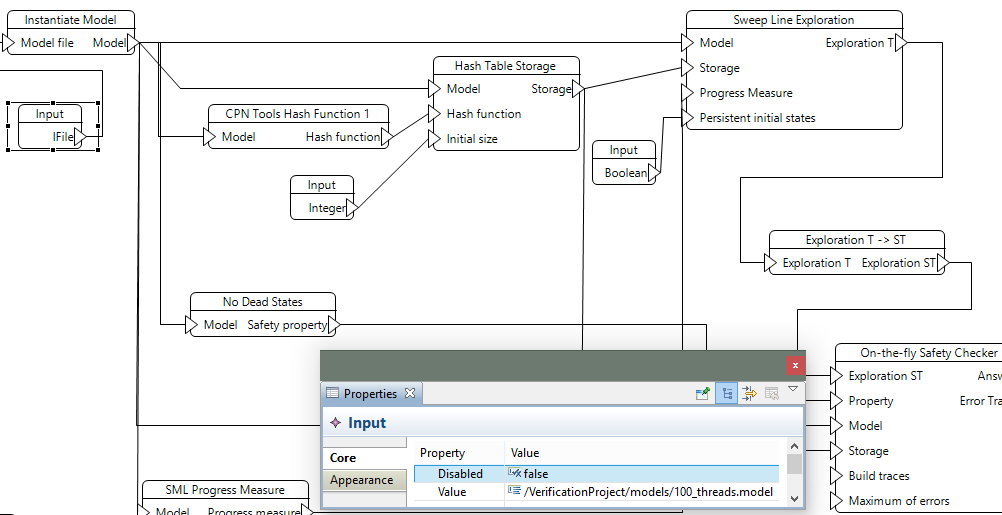
\includegraphics[width=0.5\textwidth]{./figs/sl}
	\caption{Sweep-Line Method}
	\label{fig:sl}
\end{figure}

Using the CPN Tools' built-in state space analysis tool, a bounded state space was generated reaching up-to 20 hyperperiods of component thread activity. This bounded generation took 36 minutes on a typical laptop. Our goal with such an example is to evaluate the effectiveness and utility of state space reduction techniques with respect to speed and memory usage. Figure \ref{fig:sl} shows a simple block diagram of the sweep-line method as configured in ASAP. Performing on-the-fly verification checks for lack of dead states in the analysis model, results indicate lack of system-wide deadlocks due to blocking behaviors triggered by RMI-style synchronous peer-to-peer interaction patterns. Figure \ref{fig:ds} shows analysis results obtained from a \emph{Verification Job} executed in the tool. Notice the on-the-fly verification taking less than 10 minutes to perform deadlock checks on this sample deployment. Using the \emph{Palette} in ASAP, several standard ML (SML) user queries can be created to check for domain-specific properties. 

\begin{figure}[h]
	\centering
	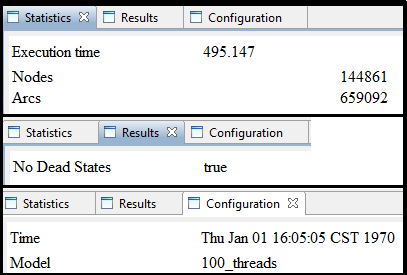
\includegraphics[width=0.4\textwidth]{./figs/asap}
	\caption{Dead States Checking in a Component-based application}
	\label{fig:ds}
\end{figure}

It must be noted here that this improved result is due to not only because of the efficient state space search but also because of symmetry-based structural reduction discussed in Section \ref{distributed_deployment}. If not for this reduction, the state space search requirements would exponentially grow for each new hardware node added to the deployment. 

\subsection{Discussion}

\subsubsection{Conservative Results}

Using estimates of worst-case execution time for component operations is motivated by the need to make exaggerated assumptions about the system behavior. Pessimistic estimates are a necessary requirement when verifying safety-critical DRE systems. Schedulability analysis with such assumptions should  provide strictly conservative results. This means that (1) if the analysis results show the possibility of a deadline violation but the deployed system does not, the obtained result is a conservative one as it assumes worst-case behavior, and (2) if the analysis results do not show any timing violations but the deployed system violates response time requirements, deadlines etc., then the analysis does not provide a conservative result and has failed to verify system behavior.

In order to guarantee conservative results, the analysis must include worst-case behaviors of all system-level threads that run at higher priority than component threads and are not necessarily modeled by the design-time tools. In our analysis, these threads are grouped into a set of critical processes with approximations made to simulate the behavior of system-level threads such as (1) globally periodic CPU utilization, (2) CPU utilization for some WCET per partition. The best approximation is chosen based on the expected behavior of such critical processes. Best-effort processes are ignored as they always run at a priority lower than the lowest-priority component thread. 
